\subsection{GFP}
    Green fluorescent protein (GFP) is protein that produces bright green fluroescence from the whole cell surface. Some cells express this protein naturally, therefore there is no need to perform cell staining or fixation in this case and the imaging can be done on living cells. Fixation of the cells is a processes of destructing their membrane and fixing them on the plate in order for the stain antibody to be able to enter the cell. The difference in DIC imaging between fixed and not fixed cells is presented in Figure \ref{fig:fixed-not-fixed}. Clearly, cell membrane is intact and clearly defined in not fixed cells, whereas in not fixed ones there is almost no definite membrane present. 
    
    Nevertheless, in order to get training data for all other targets (nuclei, ER, Golgi apparatus) the staining procedure is unavoidable. And staining requires the cells first to be fixed. That brings up the limitation of current \textit{in silico} labeling research --- cells have to be fixated in any case. DIC imaging of living and fixed cells look very different and models trained on fixed cells do not generalize well to not fixed ones. Luckily, fixing cells is not a cumbersome lab procedure and is far easier than staining the cells, which is escaped with the help of \textit{in silico} fluorescence labeling. After successfull training of the model on living GFP expressing cells, we found out that other models cannot perform that well on living cells. Therefore, the cells were fixed in order to look alike with previously acquired data and the experiments were repeated. Nevertheless, we recommend to look into the possibilities of transfer learning from fixed to live cells. The results of training on the fixated cells are presented below. 
    
    For this experiment another cell phenotype was chosen --- H19. Training the model to predict GFP fluorescence essentially allows to predict the area of the whole cell, that is used in further downstream analysis. There is no need to capture the intensities as they do not bring any useful features for selection step in CLD. However they might help for algorithms like watershed to find separate cells in order to count them. Yet the task can be simplified to predicting binary mask of GFP signal too. Binarized images are well-suited for cell area predictions. Altough one has to find a corresponding image preprocessing pipeline in order to convert training intesity fluorescence imaging into masks first. Both tranining variations are provided in this chapter --- with and without prediction of the intensities. 
    \begin{figure}[H]
        \begin{center}
            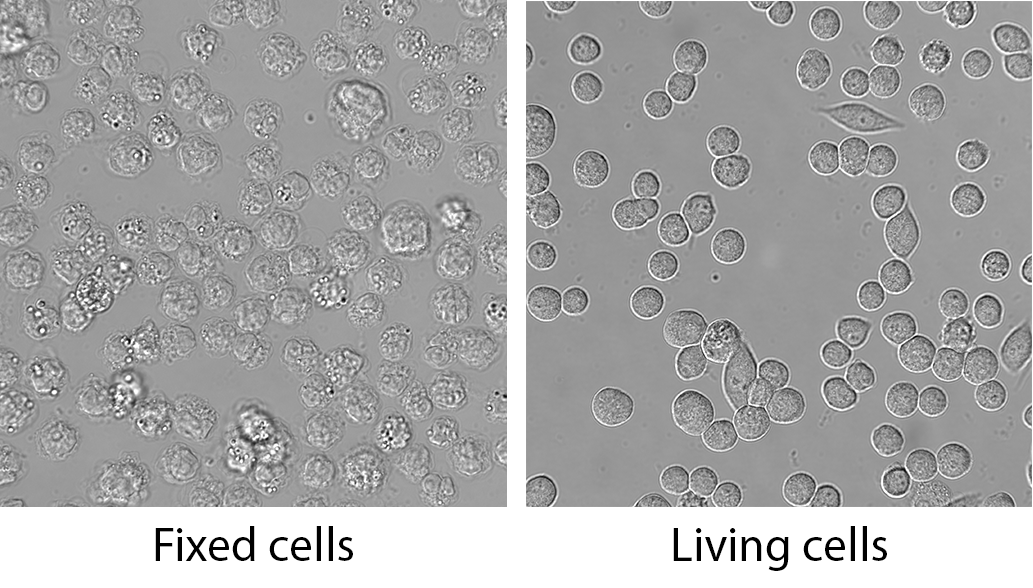
\includegraphics[width=0.5\linewidth]{bilder/gfp/fixed-not-fixed.png}
            \caption{Examples of fixed and not fixed cells DIC imaging}\label{fig:fixed-not-fixed}
        \end{center}
    \end{figure}
    \subsubsection{Preprocessing}
        \begin{figure}[H]
	\begin{center}
		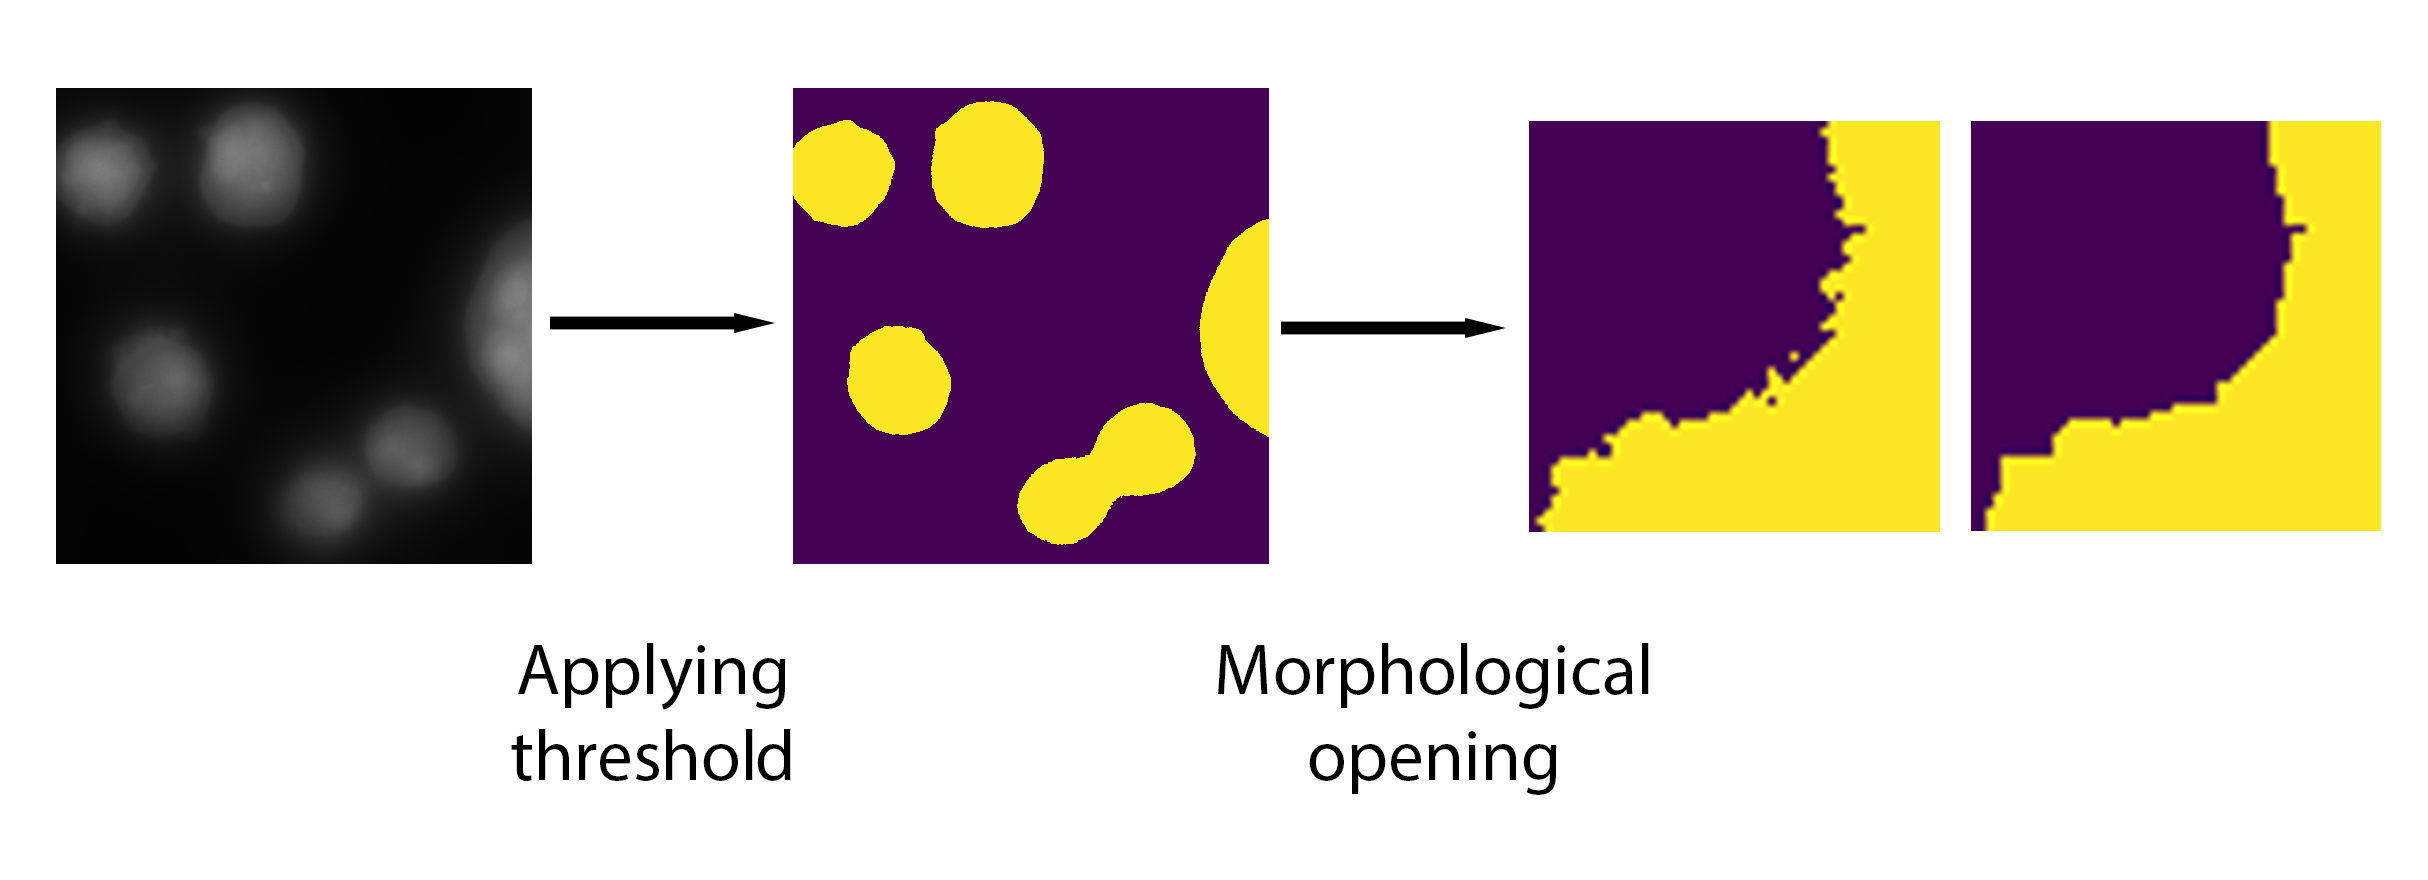
\includegraphics[width=0.5\linewidth]{bilder/gfp/binary-bce/preprocessing/preprocessing-gfp.png}
		\caption{Converting gfp to a binary mask}\label{fig:gfp-binary}
	\end{center}
\end{figure}

    \subsubsection{Predictions}
        Figure \ref{fig:gfp-pcc-predictions} presents the result of training with PCC loss on intensity images. The model convergence and visual comparison between ground truth and predictions is displayed. One can see that some of the cells are present in predictions, but are missing in ground truth images. These are dead cells that do not express GFP anymore, however the cell body is still present in DIC. Additional observation is that the boundary is generally blurry than in ground truth fluorescence, which is typical for all previous organelles as well. However all cells are clearly visible and can be separated using additional image postprocessing pipelines.
\begin{figure}[H]
	\begin{center}
		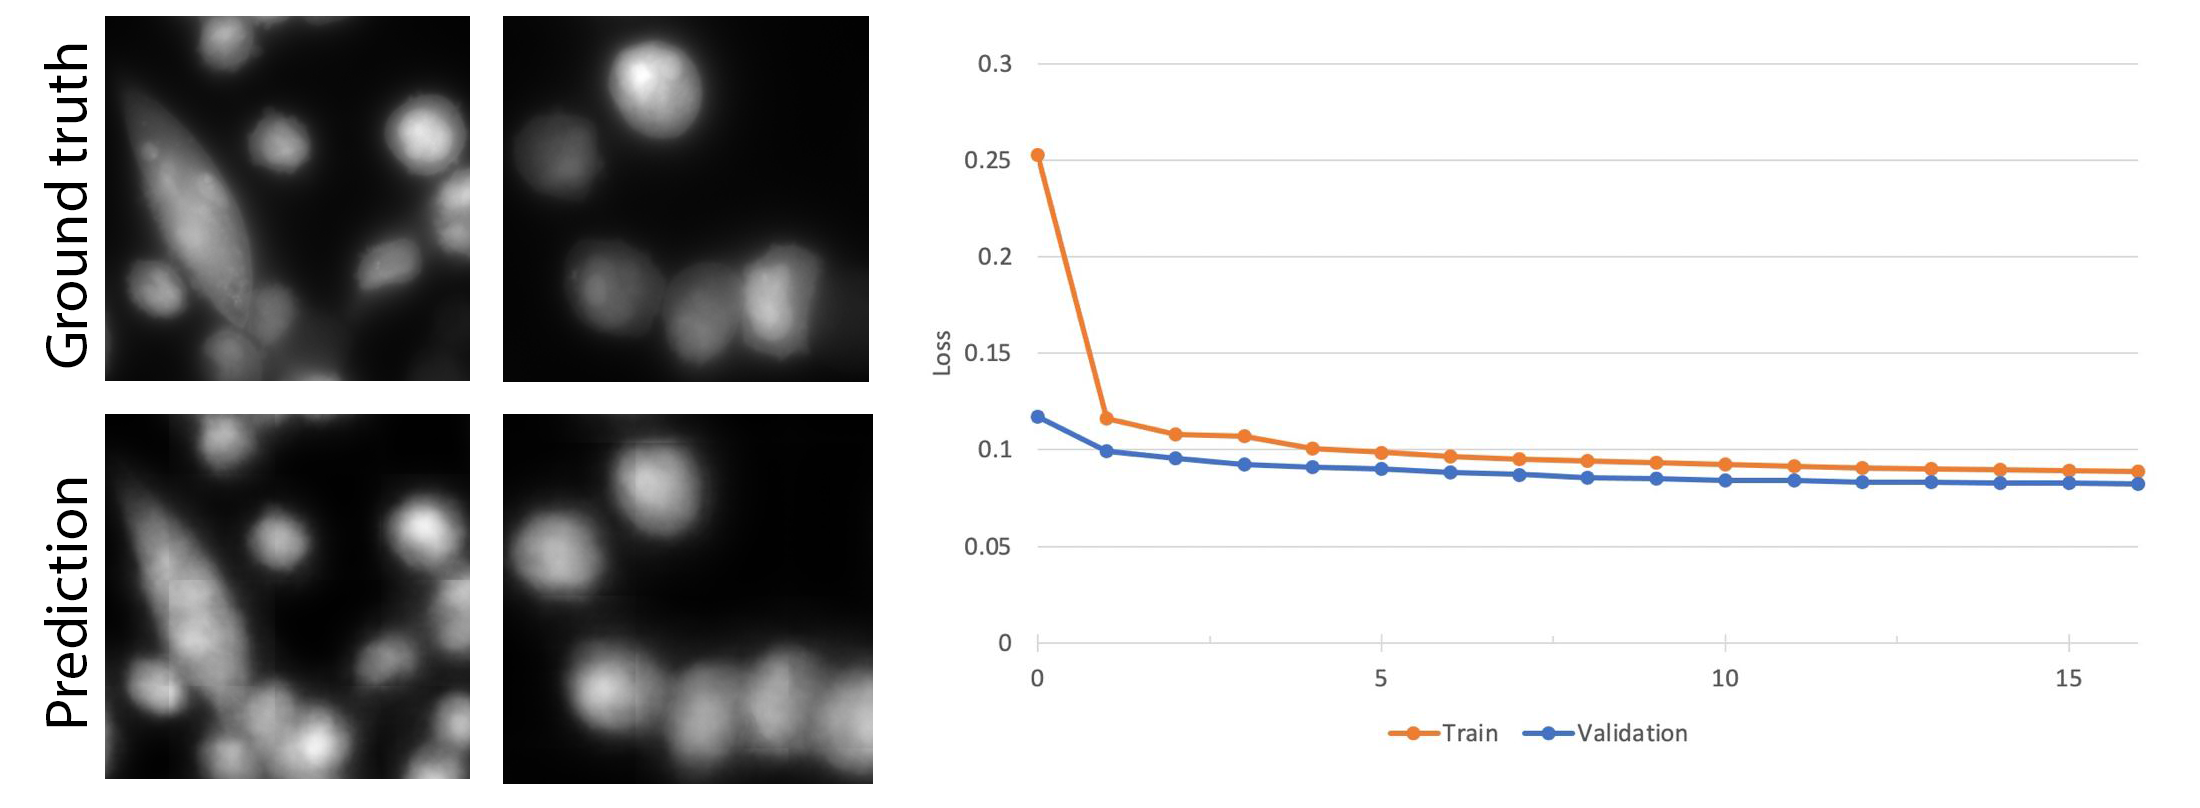
\includegraphics[width=0.9\linewidth]{bilder/gfp/predictions.png}
		\caption{Training with Pearson correlation loss}\label{fig:gfp-pcc-predictions}
	\end{center}
\end{figure}

In Figure \ref{fig:gfp-bce-predictions} one can find results of training on the binarized image dataset. Model does converge and predictions are successfull as well. Without the intensities it might be more difficult to visually separate the cells from the mask, rather then in the image with intensity values. The predicted masks are not binarized yet and contain continuous values from $[0, 1]$ interval. One can see how the model generalizes in the following observation: preprocessed ground truth image still has not very strict boundaries in its masking even after local thresholding binarization. After zooming in one can see that some cell's boundaries were oversegmented. This happens due to the different intensity values for different cells. However, this is not a an issue as the model is still able to generalize well and predicts the middle part of the cell confidently, then smoothly reduces the confidence on the cell boundary. After thresholding such predictions one can choose such a threshold that will get just enough of the cell boundary needed. In our case the value was chosen to be $0.8$.

An interesting detail here are dead cells mentioned above. They are present in DIC, but do not express GFP. One can see a clear example of such cells selected with green circles in Figure \ref{fig:gfp-bce-predictions}. The model generalizes in a way that it continues to segment all of the cells regardless of their state. This is an expected behavior as the amount of dead cells in the dataset is pretty low and ocasional mistakes do not push the model strongly enough to be able to learn the features that separate dead from alive cells. We proceed with the existing model to futher evaluation, however it might be useful for further research to address this issue. For example, \cite{Christiansen_2018} mentions the ability of their model to detect dead cells from alive by staning the dead ones and then traning the model to differentiate between them.

\begin{figure}[H]
	\begin{center}
		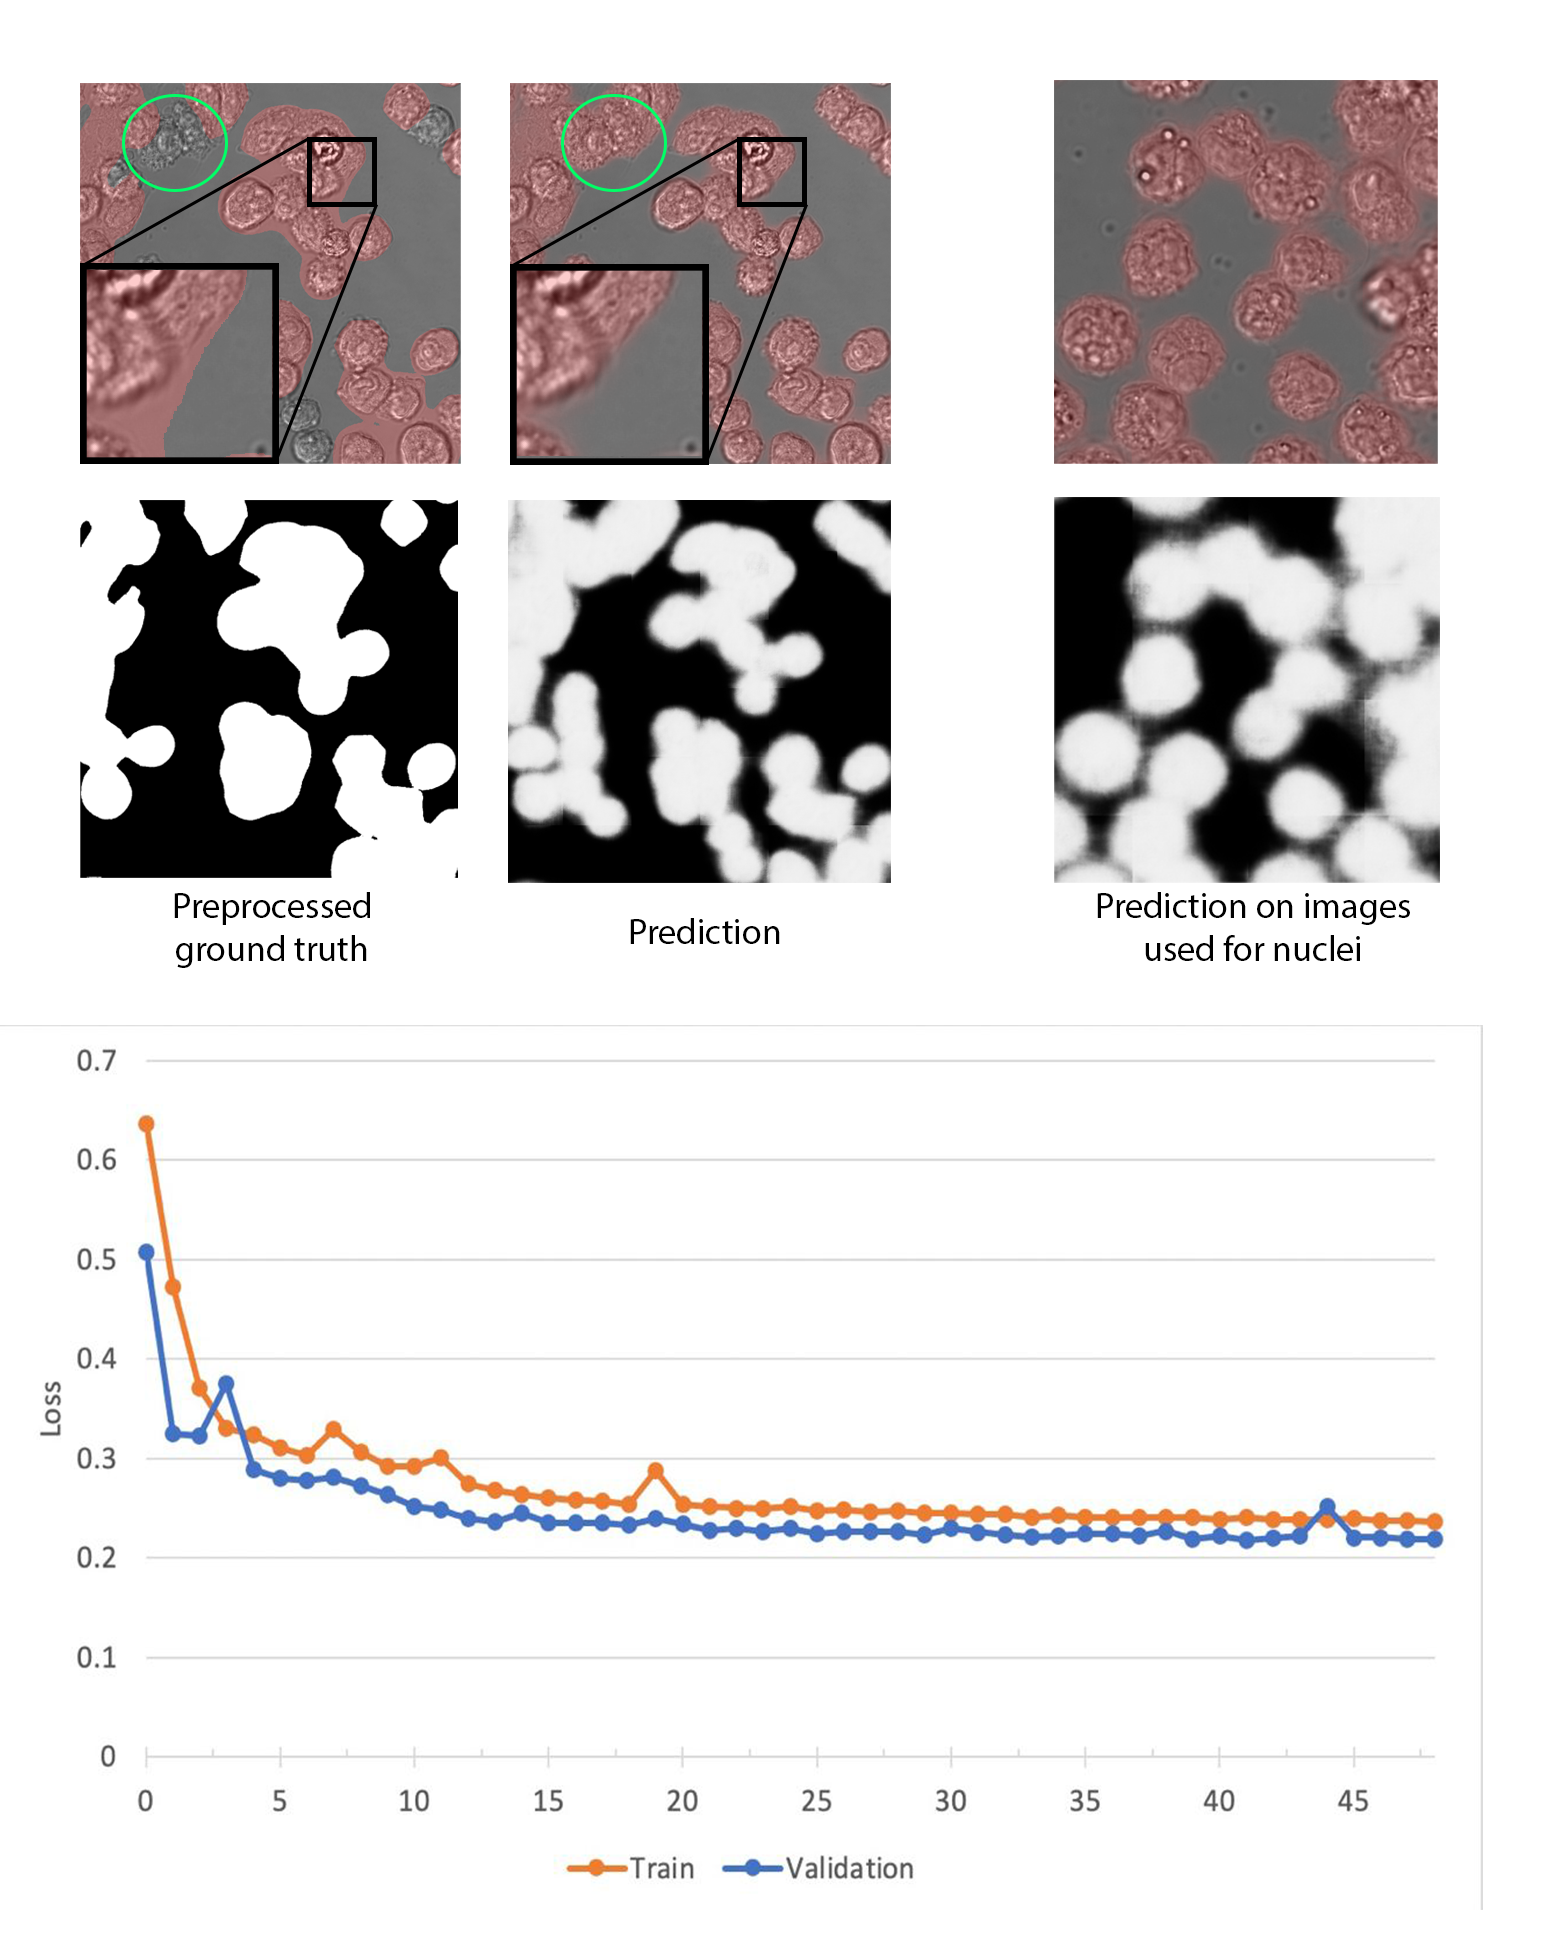
\includegraphics[width=0.7\linewidth]{bilder/gfp/binary-bce/enlarged.png}
		\caption{Training with BCE loss}\label{fig:gfp-bce-predictions}
	\end{center}
\end{figure}

    \subsubsection{Downstream metrics}
        TODO move to separate chapter?
        In this case only two metrics are important for evaluation --- the cell area and the cell count (see Table \ref{table:gfp-metrics}). Both Pearson correlation and Spearman rank coefficients are lower than in previous experiments. Influence of additional segmentation of dead cells by the model lowers correlation scores, however they still signalize the presence of a strong correlation between prediction and ground truth. 
\begin{table}[H]
    \centering
    \caption{Correlation coefficients for practical biological evaluation}
        \begin{adjustbox}{width=0.4\textwidth}
            \begin{tabular}{|c|c|c|}\hline
                BCE loss&Pearson&Spearman
                \\\hline\hline
                Number of ER&0.67&0.64\\\hline
                Area&0.82&0.75\\\hline
            \end{tabular}
            \label{table:gfp-metrics}
        \end{adjustbox}
\end{table}

Violin and scattter plots depicting the two above mentioned metrics are shown in Figure \ref{fig:gfp-bce-metrics}.
\begin{figure}[H]
	\begin{center}
		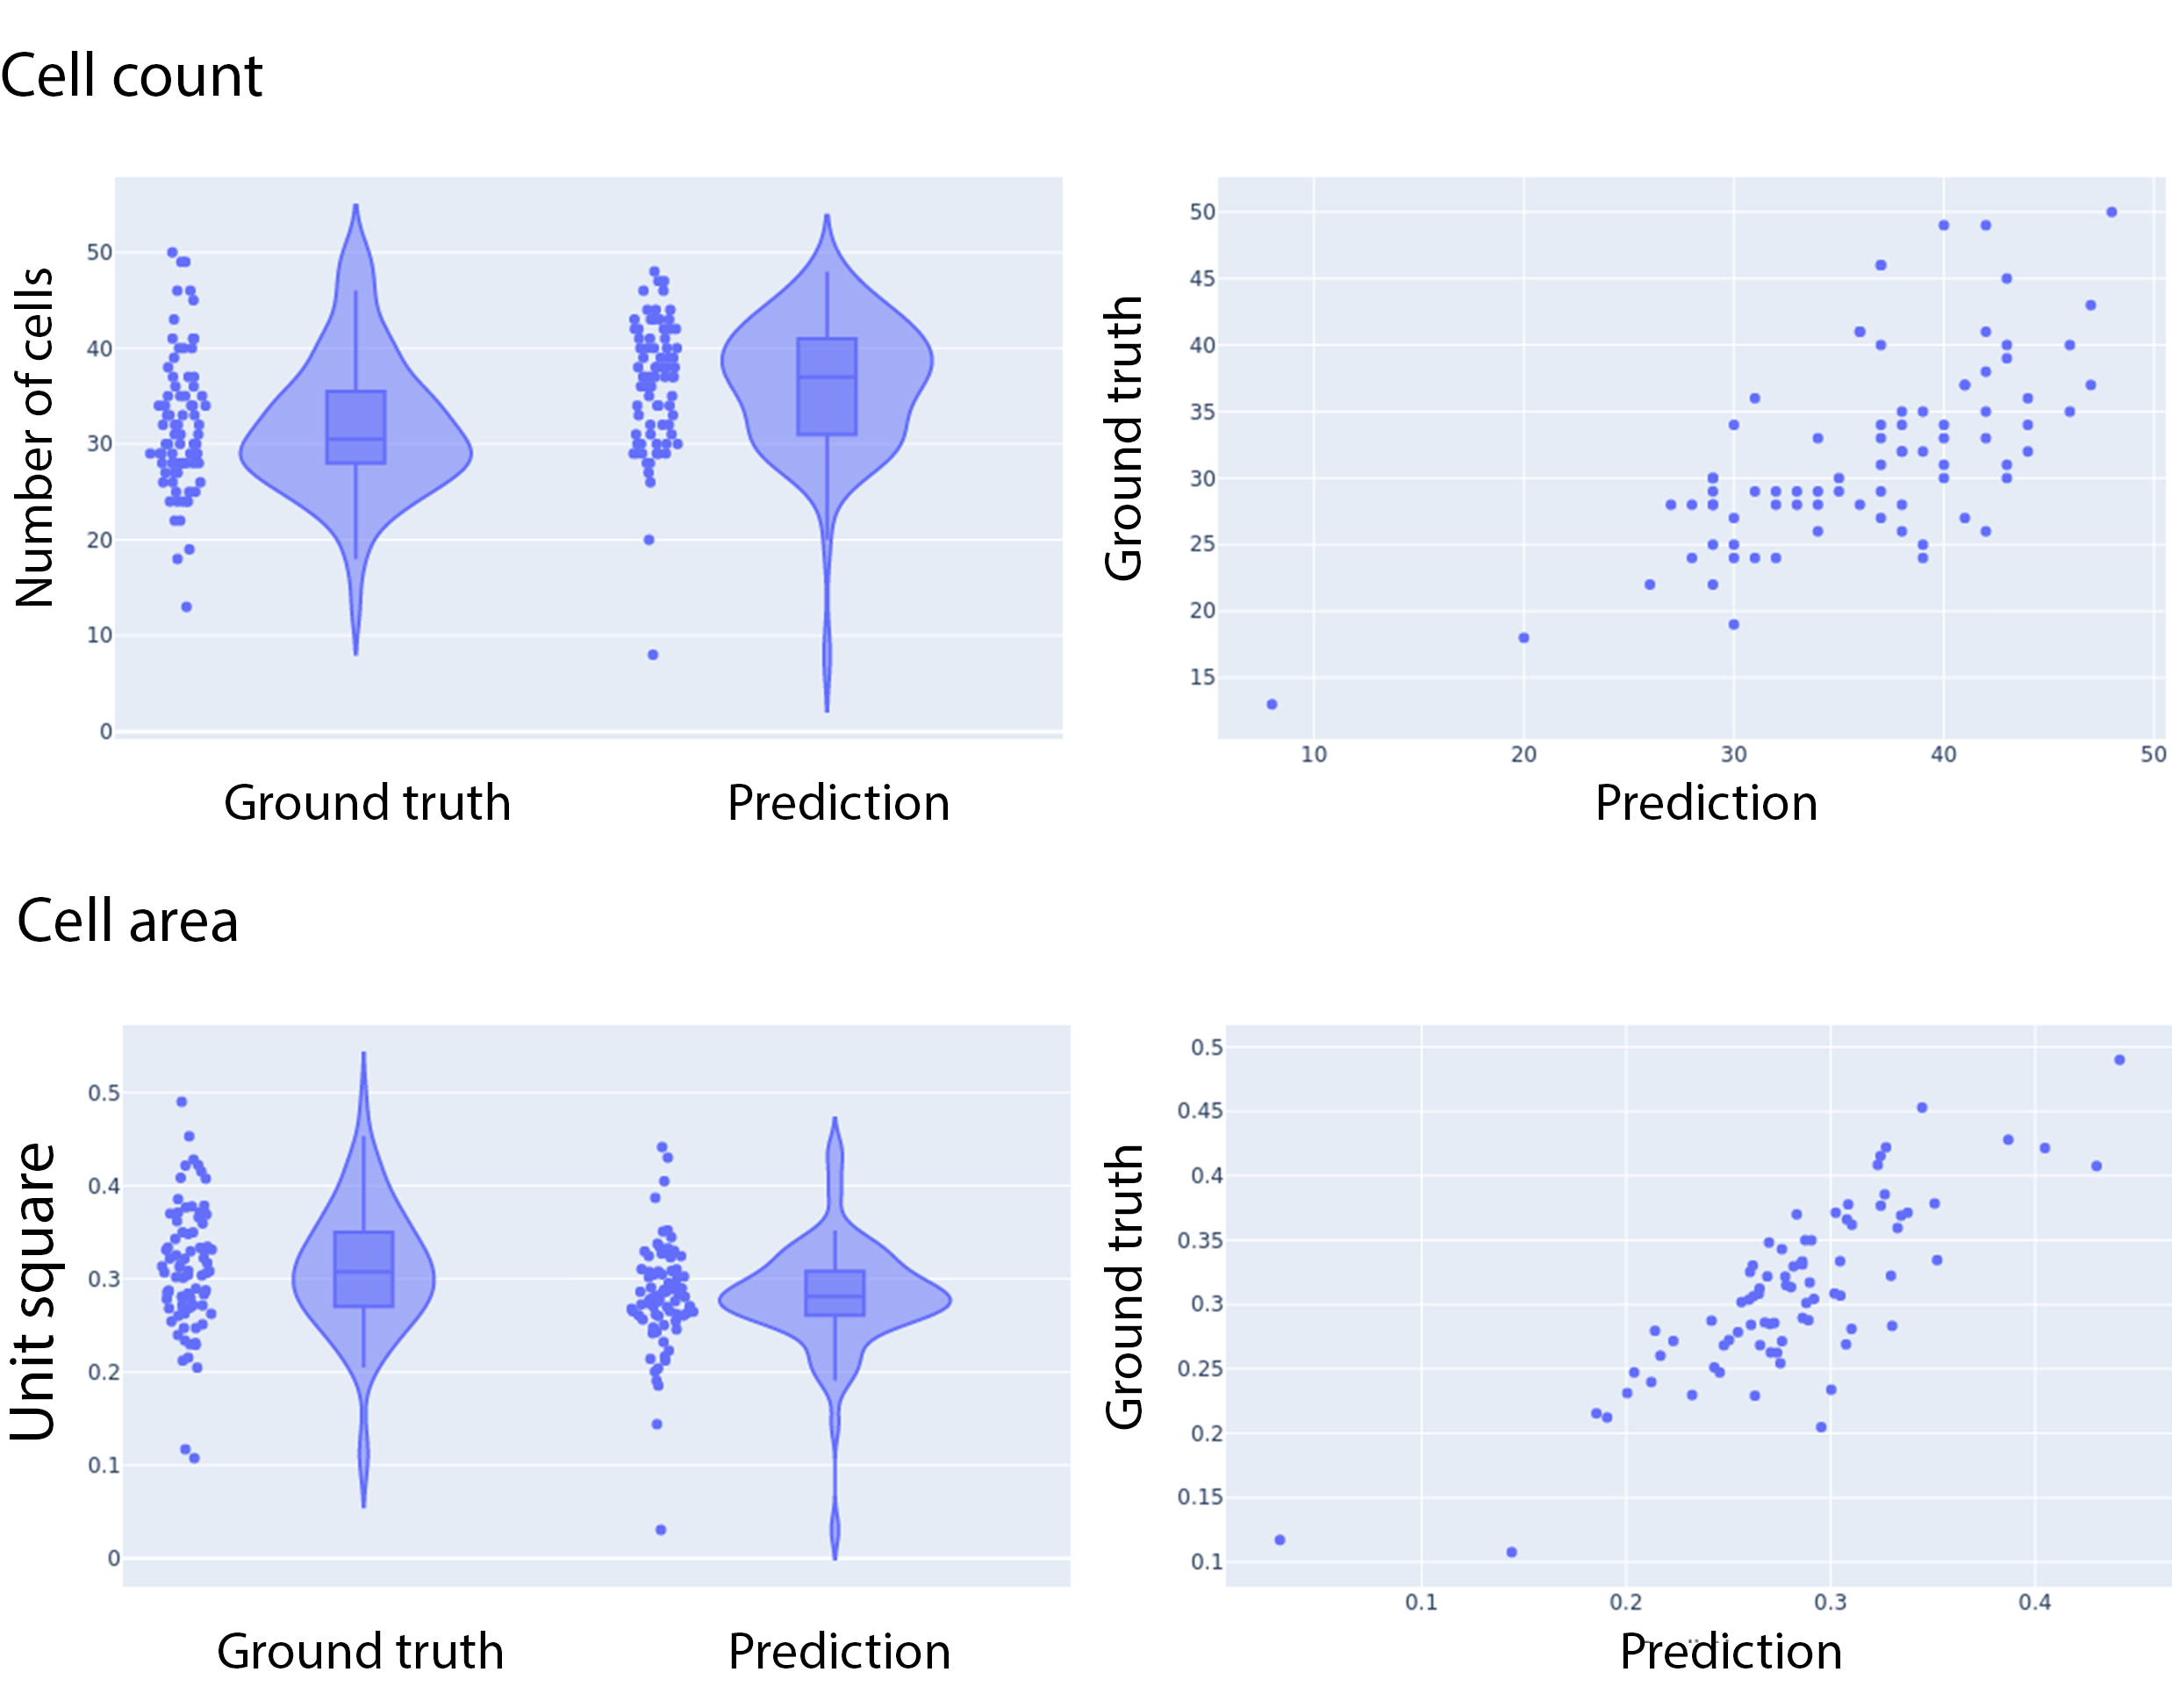
\includegraphics[width=\linewidth]{bilder/gfp/binary-bce/gfp-bce-metrics.png}
		\caption{Biological metrics}\label{fig:gfp-bce-metrics}
	\end{center}
\end{figure}
    \subsubsection{Combination of GFP, nuclei and ER}
        Now having three successful models that are able to predict GFP fluorescence from the whole cell, nuclei and ER, one can combine their predictions for the same image. To do that an output RGB image was constructed, where each prediction takes one channel. The resulting image is shown in Figure \ref{fig:combined}. Additionally one can see that the GFP model has successfully generalized on other cell phenotypes (CHOZN, PHX). Originally this model was trained on H19 phenotype only, however predictions for two other phenotypes (see Figure  \ref{fig:combined} PHX, CHOZN) highlight the cell area successfully as well.

\begin{figure}[htb]
	\begin{center}
		\includegraphics[width=0.85\linewidth]{bilder/combined/combined.png}
		\caption[GFP, Nuclei and ER combined]%
		{Combination of predictions of three UNets: GFP, nuclei and ER. Each organelle occupies one RGB channel: red --- ER, green --- GFP, blue --- nuclei.}\label{fig:combined}
	\end{center}
\end{figure}

    \subsubsection{Conclusions}
        GFP \textit{in silico} fluorescence labeling can successfully be used for counting the number of cells and estimating their size. The created models can both predict the intensity images as well as binarized masks. Intensity predictions might be more useful for the number of cells estimation as the cells better visually separate there. The models were evaluated on two biological metrics: cell size and cell count. The correlation coefficient suggests a strong correlation between the predictions and ground truth. 

The model has limitations in its ability to differentiate between dead and alive cells. This issue should be addressed in further reasearch after acquiring data for labeling dead cells. Despite the difficulty to clearly determine cell boundaries during image preprocessing for fluorescence image binarization (its overpredicting in some cases) the model can successfully generalize and predict a correct boundary for all cells. The images of not fixed cells were provided for the first time during GFP experiments and it was clear that previously trained models do not generalize on them well.  Because of this the limitation of research in terms of the cell fixation need was determined. However, it is recommended to look into possible transfer learning approaches get rid of the fixation step completely.
  
